\subsection{Spatiale Filtrering}
Et spatialt filter er også kendt som: masks, kernels, templates eller windows. Et eksempel på et spatialt filter er vist på Figur~\ref{fig:spatial-filter}.\\

\paragraph{Består af}

\begin{itemize}
	\item Et ''neighborhood'' og 
	\item En prædefineret operation.
\end{itemize}

\begin{figure}[H]
	\centering
	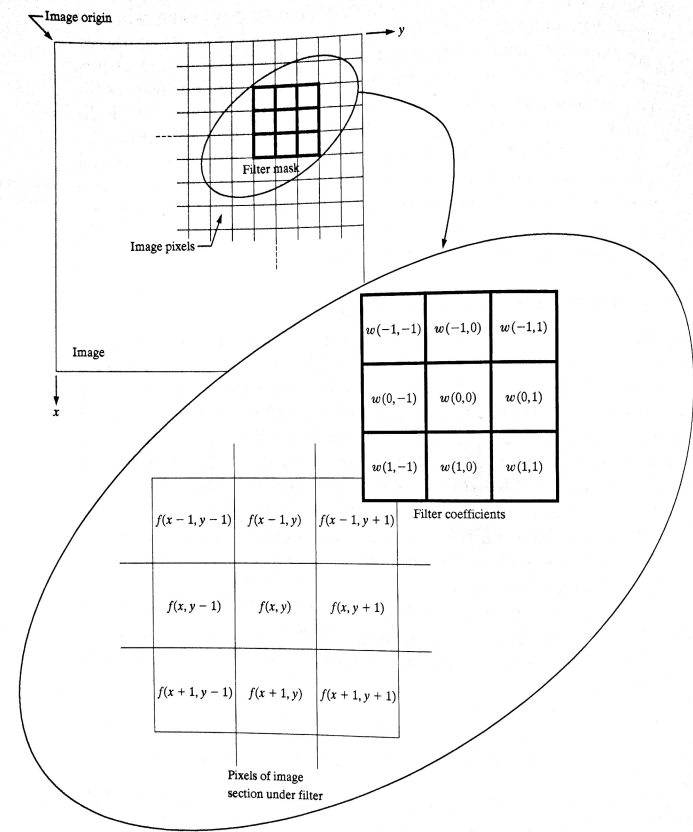
\includegraphics[width=0.8\linewidth]{figs/spm02/spatial-filter}
	\caption{Et 3 x 3 spatialt filter.}
	\label{fig:spatial-filter}
\end{figure}

Operationen er udført på de pixels der et i dette ''neighborhood''. Efter en operation er en ny pixel lavet i centeret af vores ''neighborhood''.

\subsubsection{Correlation vs. Convolution}
To meget tæt relaterede koncepter. Figur~\ref{fig:correlation-vs-convolution} viser et eksempel.

\paragraph{Correlation} er dét at bevæge et filter over billedet og beregne summen af produkter ved hver placering.

\paragraph{Convolution} er det samme, men filteret er roteret 180 grader.

\begin{figure}[H]
	\centering
	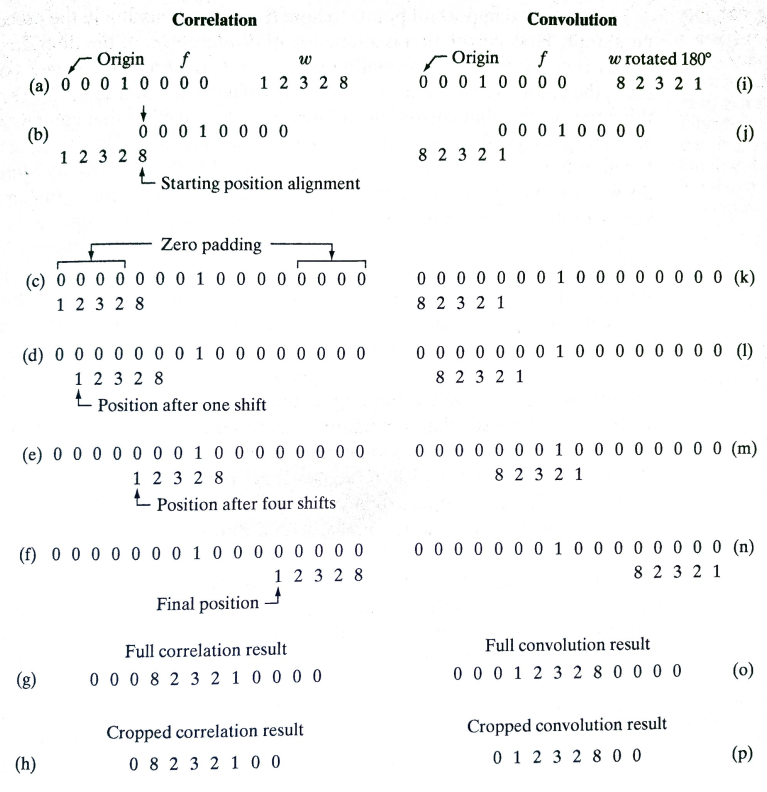
\includegraphics[width=0.9\linewidth]{figs/spm02/correlation-vs-convolution}
	\caption{Correlation vs Convolution.}
	\label{fig:correlation-vs-convolution}
\end{figure}

\subsubsection{Two important points to note}
Correlationen er en funktion af \textit{displacement} af filteret. Den firste værdi af correlationen svare til nul \textit{displacement} af filteret, og den anden til 1 unit af displacement.\\
Den anden ting er hvis vi har et filter \textit{w} og correllere denne med en funktion som består af nuller og et enkelt 1 tal\footnote{Kendt som en \textit{discrete unit impluse.}}. Så får vi en kopi af \textit{w}, som er roteret 180 grader, som vist på Figur~\ref{fig:corr-v-con}.

\begin{figure}[H]
	\centering
	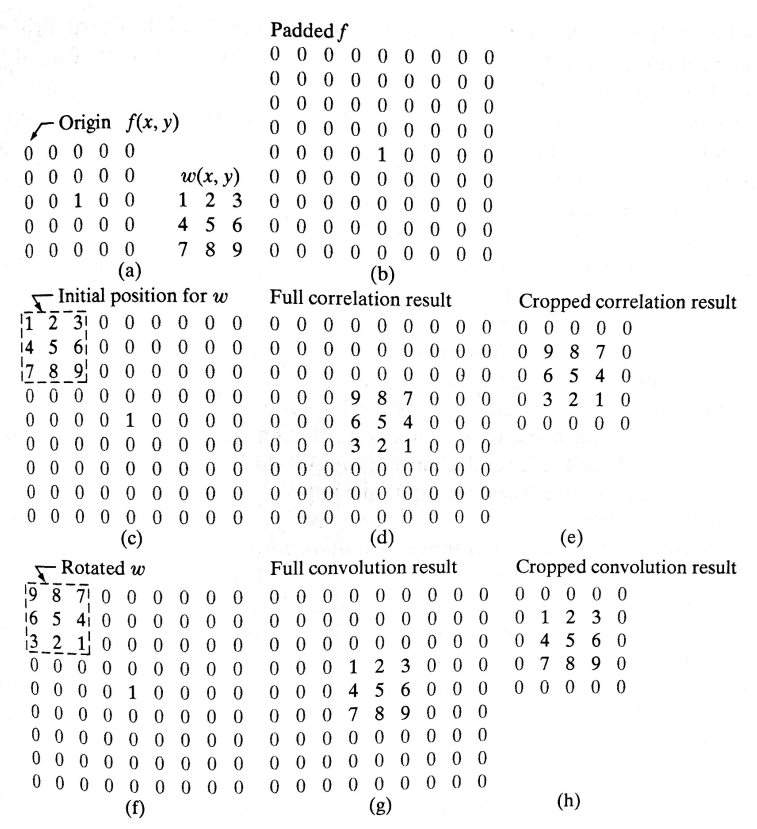
\includegraphics[width=0.8\linewidth]{figs/spm02/corr-v-con}
	\caption{Correlation (miderste række) og Convolution (nederst række).}
	\label{fig:corr-v-con}
\end{figure}

Det matematiske udtryk for correlation bliver da for et filter $w(x,y)$ af størrelse $m x n$ med et billede $f(x,y)$ til udtrykket vist på Figur~\ref{fig:correlation-eq}.

\begin{figure}[H]
	\centering
	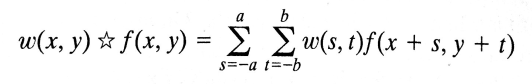
\includegraphics[width=0.6\linewidth]{figs/spm02/correlation-eq}
	\caption{Correlation matematik.}
	\label{fig:correlation-eq}
\end{figure}

Ligeledes for convolution får vi følgende udtryk vist i Figur~\ref{fig:convolution-eq}.

\begin{figure}[H]
	\centering
	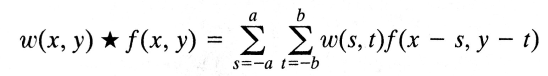
\includegraphics[width=0.6\linewidth]{figs/spm02/convolution-eq}
	\caption{Convolution matematik.}
	\label{fig:convolution-eq}
\end{figure}

I Figur~\ref{fig:correlation-eq}~og~\ref{fig:convolution-eq} skal det bemærkes at den eneste forskel er fortegnet i den sidste del af ligningen.